We use \texttt{HistGradientBoostingClassifier} as alternative to \texttt{GradientBoostingClassifier} due to computing resources constraints, and their provably near–similar performance.

\begin{table}[H]
    \centering
    \caption{\textbf{Protocol B} class–wise performance metrics across models.}
    \label{tab:cv_classwise}

    \begin{subtable}[t]{0.48\textwidth}
        \centering
        \caption{KNN}
        \label{tab:cv_knn}
        \begin{tabular}{cccc}
            \toprule
            Class & Precision & Recall & F1 Score \\
            \midrule
            NORM (0) & 64.7	& 23.7 & 34.7 \\
            MI   (1) & 19.8 & 35.6 & 25.4 \\
            STTC (2) & 18.5	& 29.3 &	22.7 \\
            HYP  (3) & 16.7 & 34.9 &	22.5 \\
            CD   (4) & 16.3	& 32.8 & 21.7 \\
            \bottomrule
        \end{tabular}
    \end{subtable}
    \hfill
    \begin{subtable}[t]{0.48\textwidth}
        \centering
        \caption{Random Forest}
        \label{tab:cv_rf}
        \begin{tabular}{cccc}
            \toprule
            Class & Precision & Recall & F1 Score \\
            \midrule
            NORM (0) & 66.0 & 76.1 & 70.7 \\
            MI   (1) & 37.0 & 27.7 & 31.7 \\
            STTC (2) & 29.6 & 23.9 & 26.4 \\
            HYP  (3) & 30.4 & 40.7 & 34.6 \\
            CD   (4) & 39.1 & 27.9 & 32.5 \\
            \bottomrule
        \end{tabular}
    \end{subtable}

    \bigskip

    \begin{subtable}[t]{0.48\textwidth}
        \centering
        \caption{Histogram–based Gradient Boosting}
        \label{tab:cv_gb}
        \begin{tabular}{cccc}
            \toprule
            Class & Precision & Recall & F1 Score \\
            \midrule
            NORM (0) & 65.1 & 87.6 & 74.7 \\
            MI   (1) & 45.9 & 26.1 & 33.2 \\
            STTC (2) & 35.7 & 16.8 & 22.7 \\
            HYP  (3) & 40.8 & 32.3 & 35.8 \\
            CD   (4) & 48.0 & 28.9 & 36.0 \\
            \bottomrule
        \end{tabular}
    \end{subtable}
    \hfill
    \begin{subtable}[t]{0.48\textwidth}
        \centering
        \caption{AdaBoost}
        \label{tab:cv_ada}
        \begin{tabular}{cccc}
            \toprule
            Class & Precision & Recall & F1 Score \\
            \midrule
            NORM (0) & 67.4 & 39.8 & 49.9 \\
            MI   (1) & 21.6 & 27.2 & 23.9 \\
            STTC (2) & 22.0 & 29.8 & 25.2 \\
            HYP  (3) & 14.8 & 62.9 & 23.9 \\
            CD   (4) & 20.3 & 25.1 & 22.3 \\
            \bottomrule
        \end{tabular}
    \end{subtable}

    \bigskip

    \begin{subtable}[t]{0.48\textwidth}
        \centering
        \caption{CatBoost}
        \label{tab:cv_cat}
        \begin{tabular}{cccc}
            \toprule
            Class & Precision & Recall & F1 Score \\
            \midrule
            NORM (0) & 66.0 & 85.0 & 74.3 \\
            MI   (1) & 44.4 & 31.0 & 36.5 \\
            STTC (2) & 35.1 & 19.0 & 24.5 \\
            HYP  (3) & 35.9 & 29.7 & 32.1 \\
            CD   (4) & 46.3 & 28.3 & 35.0 \\
            \bottomrule
        \end{tabular}
    \end{subtable}
    \hfill
    \begin{subtable}[t]{0.48\textwidth}
        \centering
        \caption{XGBoost}
        \label{tab:cv_xgb}
        \begin{tabular}{cccc}
            \toprule
            Class & Precision & Recall & F1 Score \\
            \midrule
            NORM (0) & 65.0 & 86.9 & 74.3 \\
            MI   (1) & 45.4 & 28.1 & 34.7 \\
            STTC (2) & 34.5 & 16.8 & 22.4 \\
            HYP  (3) & 40.8 & 26.6 & 32.0 \\
            CD   (4) & 45.0 & 26.6 & 33.4 \\
            \bottomrule
        \end{tabular}
    \end{subtable}
\end{table}

We present the table below to compare with their Table 12, and we complement it with a wall–clock time column, for sake of comparison against our proposed solution in \href{sec:part_2}{Part 2}.
More precisely, the time reported throughout this report refers to the time taken by the classifiers in \textbf{Protocol B}, i.e. 10–fold CV - including both training and testing, said differently, the actual inference speed is much shorter than that, and we omit the time taken by feature extractors.

\begin{table}[H]
    \centering
    \caption{\textbf{Protocol B} Performance metrics across all models.}
    \label{tab:single_model_wise}
    \begin{tabular}{ccccccc}
        \toprule
        Metrics & \texttt{XGBoost} & \texttt{RF} & \texttt{CatBoost} & \texttt{AdaBoost} & \texttt{GBoost} & \texttt{KNN} \\
        \midrule
        Precision & 46.1 & 40.4 & 45.5 & 29.2 & 47.1 & 27.2 \\
        Recall & 37.0 & 39.3 & 38.6 & 37.0 & 38.3 & 31.2 \\
        F1 Score & 39.4 & 39.2 & 40.5 & 29.0 & 40.5 & 25.4 \\
        Accuracy & 59.0 & 54.6 & 59.0 & 35.6 & 59.6 & 27.7 \\
        \midrule
        \midrule
        Time (s) & 49.5 & 57.2 & 282.7 & 322.2 & 140.7 & 2.3 \\
        \bottomrule
    \end{tabular}
\end{table}

\begin{figure}[H]
    \centering
    \caption{\textbf{Protocol A} Confusion matrices of all classifiers.}
    \label{fig:reproduced_confusion}
    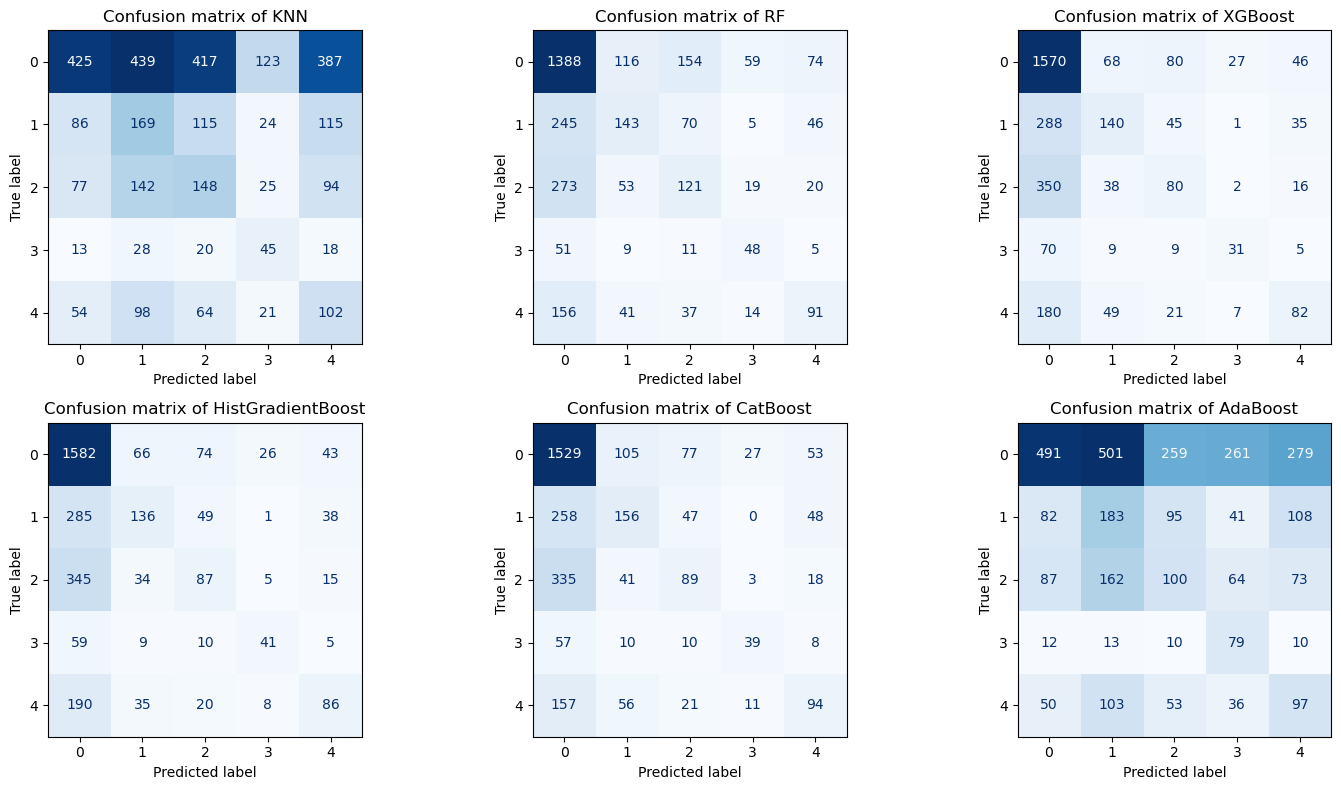
\includegraphics[width=\textwidth]{figures/part1/reproduced_confusion.png}
\end{figure}

\begin{figure}[H]
    \centering
    \caption{\textbf{Protocol A} ROC–AUC curves and scores across classifiers.}
    \label{fig:reproduced_roc}
    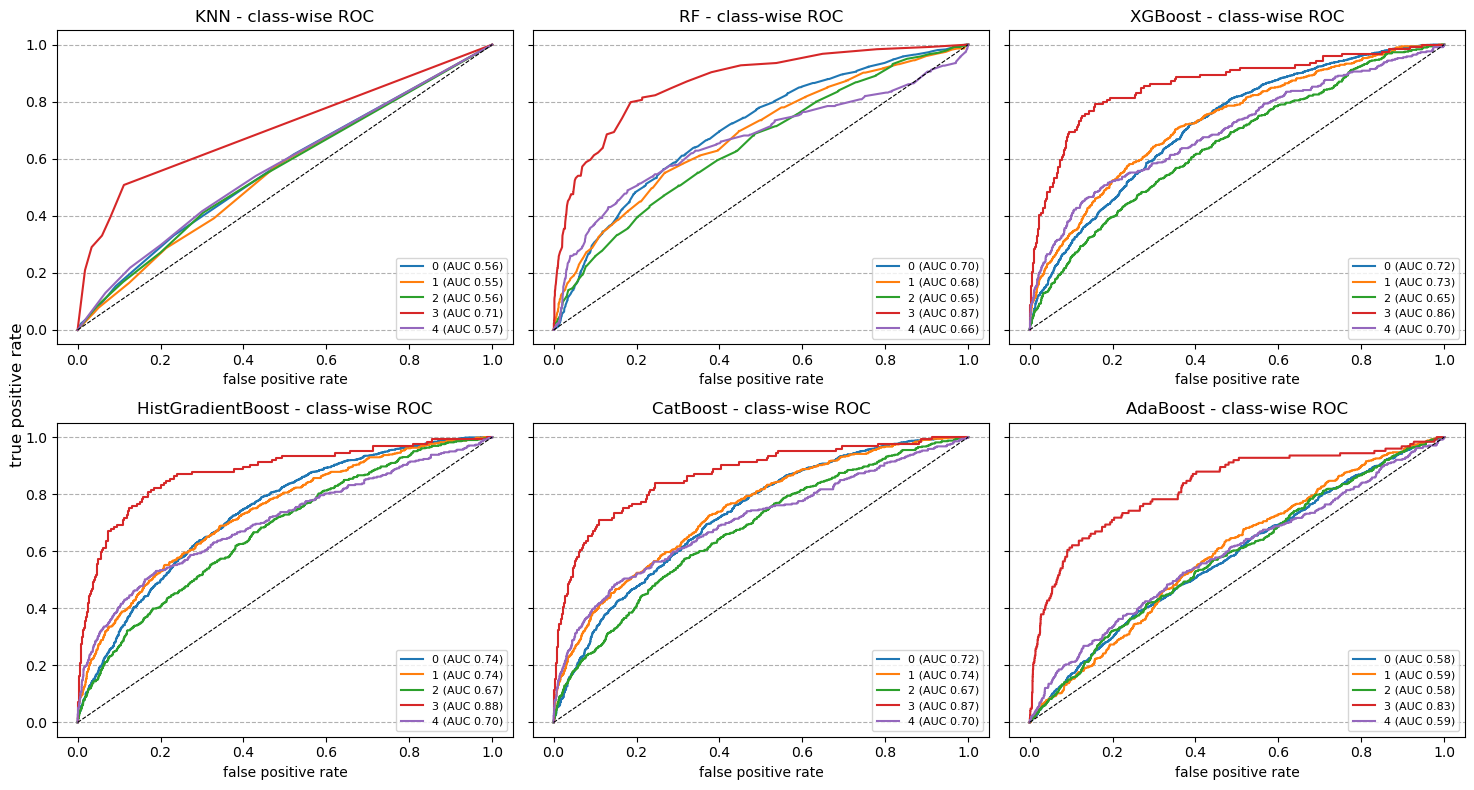
\includegraphics[width=\textwidth]{figures/part1/reproduced_roc_curve.png}
\end{figure}